\documentclass[10pt,a4paper]{article}
\usepackage[utf8]{inputenc}
\usepackage[spanish]{babel}
\usepackage{amsmath}
\usepackage{amsfonts}
\usepackage{amssymb}
\usepackage{cite}
\usepackage[]{algorithm2e}
\usepackage{graphicx}
\author{Jon Goenetxea}
\title{Heuristicos de Búsqueda}
\begin{document}

\maketitle

\begin{abstract}
En este trabajo se presenta una comparativa entre dos diferentes algoritmos de búsqueda heuristica. El primero, denominado \textit{Hill Climbing}, es un algoritmo basado en búsqueda local, que se ha implementado utilizando múltiples inicializaciones (\textit{multi-start}) para tratar de evitar los mínimos locales. Como segundo algoritmo para la comparación se ha escogido un algoritmo genético, que entra dentro de los algoritmos tipificados como poblacionales. En el apartado experimental, se han analizado las posibles configuraciones para la búsqueda local, y se ha hecho una comparación utilizando un test de hipótesis de Wilcoxon.
\end{abstract}

\section{Problema de asignación cuadrática}
\label{sec:planteamiento}
El problema de la asignación cuadrática, que se denota por sus siglas en inglés \textit{QAP} (\textit{Quadratic assignment problem}), fue planteado como un modelo matemático para un conjunto de actividades económicas indivisibles. Posteriormente fue demostrado que QAP pertenece a los problemas no polinomiales duros, y es aplicable a un sin número de situaciones.

La primera vez que este problema fue planteado fue en 1957 por Kooppmnans y Beckmann. En 1976, Sahni y Gonzalez demostraron que era un problema NP duro 
%\cite{Sahni:1976:PAP:321958.321975}
.

Este tipo de problemas consisten en escoger para N localizaciones la distribución de N instalaciones que minimice el coste de instalación. Para la toma de decisiones hay que tener en cuenta dos factores principales: 1) el coste de moverse entre localizaciones (distancias, coste de transporte, penalizaciones, etc.), y 2) el flujo de material entre instalaciones.

Para definir estos datos, se definen dos matrices (la matriz de distancias y la matriz de flujos de material) que modelan el comportamiento del sistema de instalaciones. La matriz de distancias se define como $D=[d_{ij}]$, donde $d_{ij}$ representa el coste de transporte de la localización $i$ a la localización $j$. La matriz de flujos se define como $F=[f_{kl}]$, que representa el flujo de material entre la instalación $k$ a la instalación $l$.

Cada configuración (una posible ubicación para todas las instalaciones) se representa en forma de permutación (ver ecuación \ref{eq:elementRepresentation}).
\begin{equation}
\sigma = (\sigma_1\sigma_2\sigma_3...\sigma_n)
\label{eq:elementRepresentation}
\end{equation}

La función de coste a minimizar por lo tanto, tendrá en cuenta el coste de transporte dependiendo del flujo entre las instalaciones y la distancia entre las localizaciones. Esta función se puede modelar como muestra la ecuación \ref{eq:costFunction}.
\begin{equation}
f(\sigma)=\sum^n_{i=1}\sum^n_{j=1}d_{\sigma(i)\sigma(j)}f_{ij}
\label{eq:costFunction}
\end{equation}

\section{Propuestas de solución basadas en búsqueda local}
Como se ha presentado anteriormente, el algoritmo implementado para la búsqueda local es el \textit{Hill Climbing}. Es un algoritmo de búsqueda local sencillo. Se basa en analizar los resultados vecinos de una muestra, en busca de un resultado mejor que el actual. Esto se hace iterativamente, por lo que el caer en un óptimo local es muy probable. Para minimizar el caer en óptimos locales, se toman varias medidas.

La primera medida se trata hacen varias reinicializaciones (conocido como \textit{multi start}) utilizando el mejor de los resultados como respuesta final. Dentro de cada iteración, y con el fin de salir de un mínimo local, se generan varias muestras aleatorias y se compara si alguna de ellas es mejor que la candidata actual.

El pseudo-código general para este algoritmo sería el siguiente:

\begin{algorithm}[H]
 \KwData{cantidad de 'start'-s, función de coste}
 \KwResult{valor de error mínimo encontrado}
 \For{cada 'start'}{
 generar permutación inicial con función aleatoria\;
 \While{no se ha encontrado mínimo local}{
  escoger candidato\;
  \While{no encontremos mejor vecino}{
	  calcular nuevo vecino\;
	  evaluar vecino\;
	  \If{nuevo vecino mejora}{
   		guardar nuevo vecino como actual\;
   		no se ha encontrado mínimo local\;
   		}
  }
 }
 }
 devolver valor de mejor permutación encontrada
 \caption{Pseudocódigo de \textit{Hill Climbing} modificado.}
\end{algorithm}

Este algoritmo tiene pocos parámetros para configurar, lo que simplifica su configuración. El único parámetro que es necesario definir para su implementación general es la cantidad de inicializaciones a hacer. No obstante, y con el fin de reducir el tiempo de ejecución, se definen varios límites para la ejecución. Estos límites se listan en la tabla \ref{tab:lsParameters}. Además de esta configuración, es necesario definir el método de calcular los vecindarios, y hay que escoger uno que se adecue al problema. 

\begin{table}
\begin{center}
\begin{tabular}{|c||c|}
\hline
Parámetro & Valor \\
\hline \hline
Tamaño multistart & 15 \\
\hline
Número máximo de evaluaciones & 150 \\
\hline
Número de muestras aleatorias tras mínimo local & 3\\
\hline
Número máximo de vecinos analizados & Todos\\
\hline
\end{tabular}
\end{center}
\caption{Lista de parámetros de configuración para el algoritmo de búsqueda local.}
\label{tab:lsParameters}
\end{table}

En este aspecto se han analizado dos sistemas de vecinos diferentes: \textit{Swap} y \textit{2-opt}.
El sistema de vecinos \textit{Swap} consiste en generar vecinos cambiando un elemento de la lista con otro. Si intercambiamos un elemento al azar con cada uno de los demás, generamos un vecindario con \textit{n} vecinos.
El sistema de vecinos \textit{2-opt} consiste en intercambiar dos elementos en la lista de elementos. Si se tienen en cuenta todas las posibles permutaciones, se consigue un vecindario de \textit{k} elementos, donde \textit{k} se calcula con la ecuación \ref{eq:2optNeigbor}.

\begin{equation}
\label{eq:2optNeigbor}
k = \frac{n*(n-1)}{2}-n
\end{equation}

En los experimentos, se ha comprobado que el algoritmo \textit{2-Opt} es más efectivo a la hora de acercarse a la solución óptima, pero el tiempo de computo también es significativamente mayor que el del método \textit{Swap}. Por ello, se ha optado por utilizar el método \textit{Swap}, modificando la ejecución para que pare de calcular el vecindario en el momento en el que se encuentre un vecino que mejore el valor actual.

\begin{figure}[!htb]
\minipage{0.32\textwidth}
  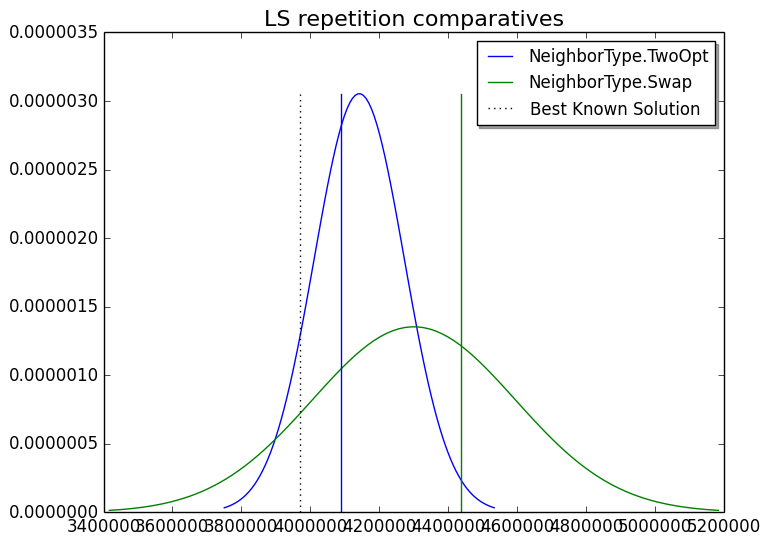
\includegraphics[width=\linewidth]{optSwapComparative.png}
\endminipage\hfill
\minipage{0.32\textwidth}
  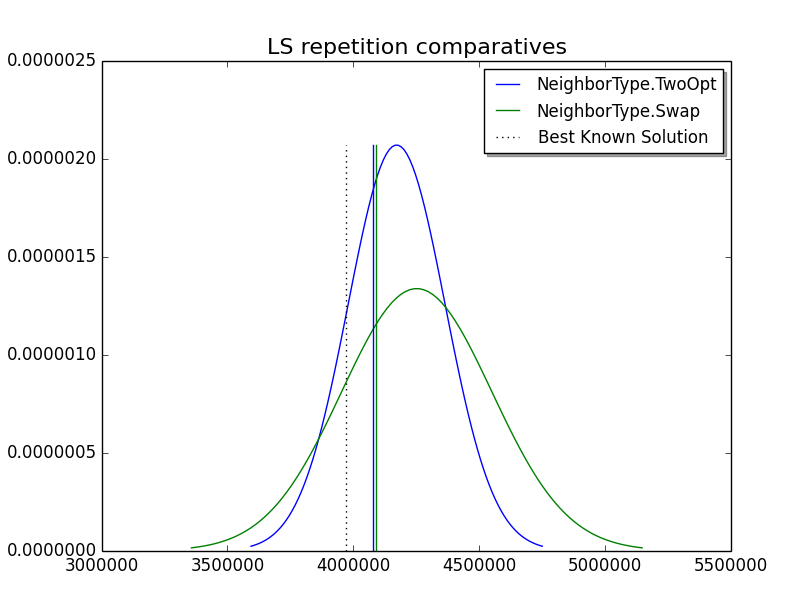
\includegraphics[width=\linewidth]{optSwapComparative_2.png}
\endminipage\hfill
\minipage{0.32\textwidth}
  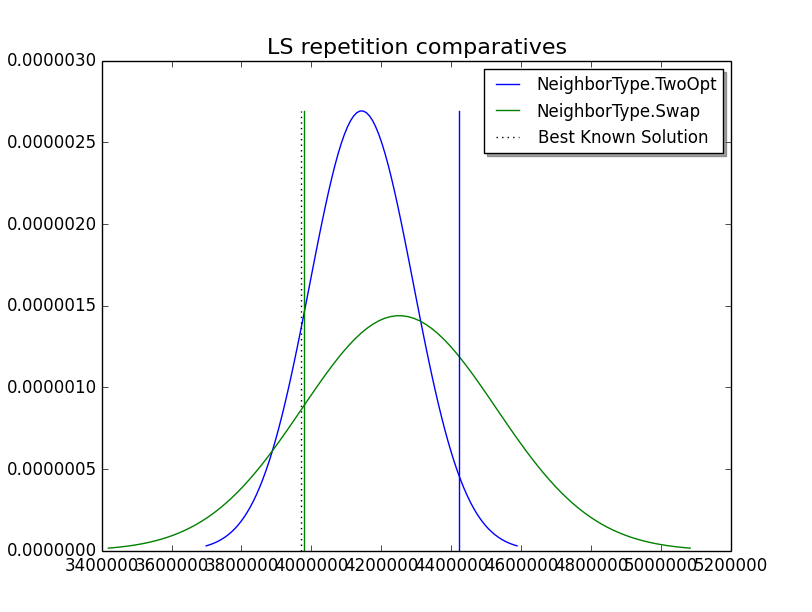
\includegraphics[width=\linewidth]{optSwapComparative_3.png}
\endminipage
\caption{3 ejecuciones comparativas entre 2-Opt y Swap, con 30 repeticiones cada una y cogiendo los mejores resultados en cada una. La línea vertical representa el valor mínimo para cada algoritmo, y la curva representa la distribución normal teniendo en cuenta la media y la varianza de los mejores resultados de las 30 ejecuciones.}
\label{fig:optSwapComparison}
\end{figure}


\section{Propuestas de solución basadas en algoritmos poblacionales}
El algoritmo poblacional implementado es un algoritmo genético. Este algoritmo se basa en las teorías clásicas de la evolución darwiniana como base para generar una serie de iteraciones que generan una población mejor que la generación anterior.

Un algoritmo genético consta de cuatro fases principales: 1) evaluación (evaluation), 2) selección (selection), 3) cruce (crossover) y 4) mutación (mutation). Cada iteración genera una nueva generación después de pasar por todos estos estados. Se puede poner un criterio de terminación, con el que podemos decidir si la generación actual es ya lo suficientemente buena para el resultado, o si se han utilizado los recursos asignados, por ejemplo. La figura \ref{fig:gaIteration} muestra gráficamente la secuencia de estados de una iteración.

\begin{figure}[h]
\centering
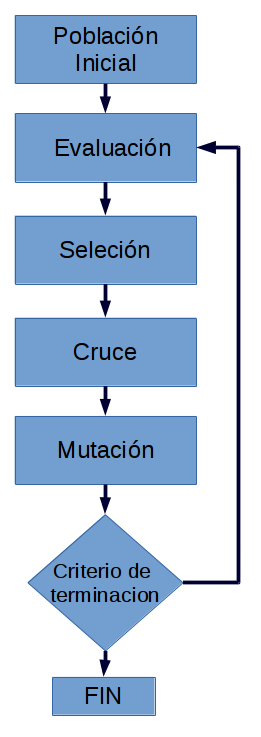
\includegraphics[scale=0.4]{GaIteration.png} 
\caption{Secuencia de una iteración de un algoritmo genético.}
\label{fig:gaIteration}
\end{figure}



\subsection{Fase de Evaluación}
En la fase de evaluación se evalúan todos los individuos de la población actual. Esto se hace utilizando la función de coste que se ha expuesto en el apartado \ref{sec:planteamiento}.

Por lo tanto, cada individuo tendrá asociado el valor de su resultado, dando un indicador de la "calidad" de dicho individuo.

\subsection{Fase de Selección}
En la fase de selección se escogen los individuos de la población con mejores resultados. 
Para ello se pueden utilizar diferentes opciones. Entre ellas se ha escogido la \textit{selección por torneo}. 

Esta selección se realiza mediante una comparación entre un subconjunto de individuos de tamaño concreto (definido como parámetro), escogidos al azar dentro de la población.

Este tipo de selección se efectúa de manera muy rápida dado que no es necesario evaluar la totalidad de la población. No obstante, hay que definir un nuevo parámetro por lo que añade complejidad a la configuración.

\subsection{Fase de Cruce}
En esta fase, se unen y combinan los diferentes individuos en el subconjunto de \textit{mejores} individuos. Es necesario encontrar una función de cruce que genere nuevos individuos aprovechando las cualidades de los originales, y tratando de transmitirlas a las nuevas generaciones. Para esta fase, se han barajado varias opciones. 

La primera de ellas, combina dos individuos por mitades. Es decir, coge la primera mitad de un individuo A, y la segunda mitad de un individuo B. Los nuevos individuos (denominados A' y B') tendrán la primera parte de A y la segunda de B respectivamente. Para rellenar la mitad restante, lo que se hace es colocar los valores que faltan por incluir con el mismo orden que aparece en el individuo original. Por lo tanto, A' tendrá la primera mitad de A, y los elementos restante en el mismo orden que aparecen en B, y B' tendrá la segunda mitad de B y los demás valore en el mismo orden que aparecen en A.

Como segunda opción, se ha planteado una función en la que se intercambia un elemento al azar entre los dos individuos. Es decir, se escoge un índice al azar (por ejemplo 2) y se coloca el valor en 2 de A en la posición 2 de B, y viceversa. Esta acción por si sola es probable que duplique valores en el nuevo individuo. Para evitar esto, el antiguo valor en la posición 2 se coloca en el lugar en el que está el valor que se va a insertar. La figura \ref{fig:gaCrossover} representa gráficamente el proceso de cruce descrito.

\begin{figure}[h]
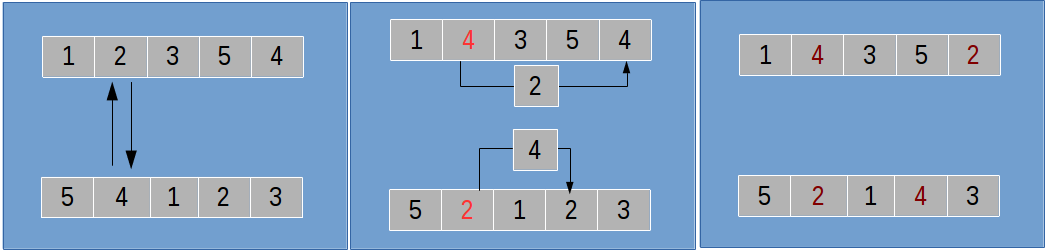
\includegraphics[scale=0.45]{gaCrossover.png} 
\caption{La figura muestra de forma gráfica el proceso de cruce escogido para el algoritmo genético. En el primer paso (izquierda), se seleccionan los elementos con un índice escogido al azar. En el segundo (centro), se intercambia el elemento entre los dos individuos, y se detecta la posición del número que va a ser sustituido. El tercer paso (derecha), se pueden ver los nuevos individuos, y como no tienen repeticiones.}
\label{fig:gaCrossover}
\end{figure}

\subsection{Fase de Mutación}
Para aumentar la variedad de posibilidades, se añade un factor de mutación. Este factor hace que una parte de la población mute (tenga un cambio adicional) en cada iteración. Con esto conseguimos configuraciones que no estuviesen en la generación anterior, y que la fase de cruce no puede generar.

La función de mutación escogida es la de intercambiar 2 elementos del individuo. Para ello, se escogen dos índices al azar, y se intercambian los elementos.

Esta fase añade un elemento a configurar, que es la probabilidad de mutación de un individuo.

\subsection{Configuración final}
A diferencia del algoritmo de \textit{Hill Climbing}, este tipo de algoritmos tiene más parámetros que definir. La tabla \ref{tab:gaParameters} lista los parámetros escogidos para este algoritmo.

\begin{table}
\begin{center}
\begin{tabular}{|c||c|}
\hline
Parámetro & Valor \\
\hline \hline
Tamaño población & 150 \\
\hline
Número de generaciones & 15 \\
\hline
Factor Mutación & 0.05\\
\hline
Tamaño subconjunto torneo & 3\\
\hline
Factor de cruce & 0.5 \\
\hline
\end{tabular}
\end{center}
\caption{Lista de parámetros de configuración para el algoritmo genético.}
\label{tab:gaParameters}
\end{table}

Se ha definido el número de generaciones para que sea el mismo que la cantidad de iteraciones que se realizan en el algoritmo de búsqueda local. En este sentido, tanto el algoritmo de búsqueda local realizará $n$ iteraciones, y el algoritmo genético creará a su vez $n$ generaciones para lograr el resultado final. 

\section{Experimentación}


\section{Conclusiones}


\bibliography{referencies}{}
\bibliographystyle{plain}

\end{document}